\documentclass[svgnames,11pt]{beamer}
\input{/home/tof/Documents/Cozy/latex-include/preambule_commun.tex}
\input{/home/tof/Documents/Cozy/latex-include/preambule_beamer.tex}
%\usepackage{pgfpages} \setbeameroption{show notes on second screen=left}
\author[]{Christophe Viroulaud}
\title{Tris}
\date{\framebox{\textbf{Algo 04}}}
%\logo{}
\institute{Première - NSI}

\begin{document}
\begin{frame}
    \titlepage
\end{frame}
\begin{frame}
    \frametitle{}

    \begin{center}
        \centering
        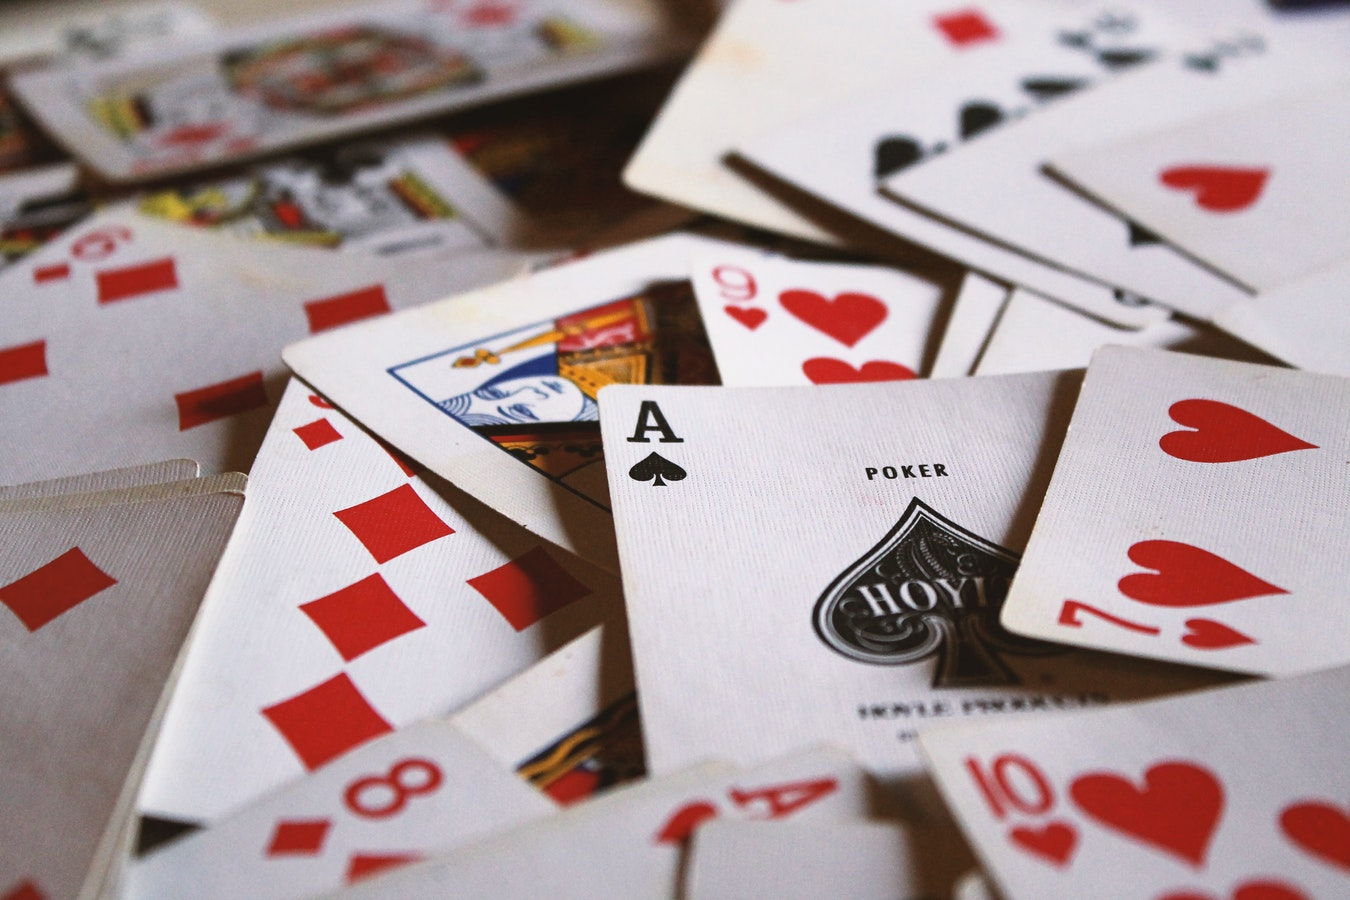
\includegraphics[width=8cm]{ressources/cartes.jpg}
        \captionof{figure}{Trier un jeu de cartes est un problème informatique.}
        \label{IMG}
    \end{center}

\end{frame}
\begin{frame}
    \frametitle{}

    \begin{framed}
        \centering Déterminer plusieurs méthodes de tris de données.
    \end{framed}

\end{frame}
\section{Algorithmes de tris}
\subsection{Recherche}
\begin{frame}
    \frametitle{Algorithmes de tris - Recherche}
    \begin{center}
        \centering
        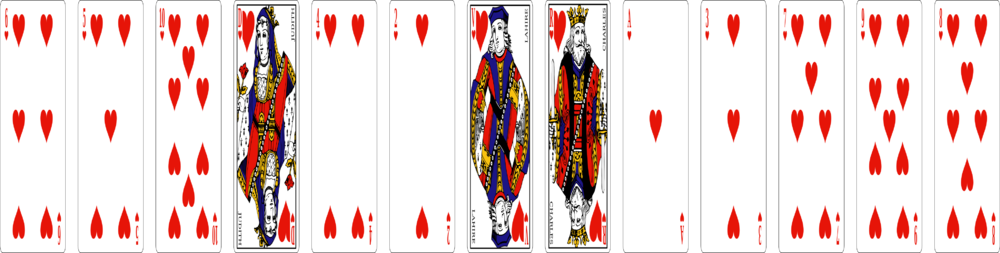
\includegraphics[width=10cm]{ressources/jeu-coeur-melange.png}
    \end{center}
    \begin{activite}
        \begin{enumerate}
            \item Prendre le paquet de cartes mélangées et les étaler sur la table.
            \item Trier les cartes.
            \item Formaliser la méthode utilisée sous forme d'un algorithme.
        \end{enumerate}
    \end{activite}

\end{frame}
\subsection{Tri par sélection}
\begin{frame}
    \frametitle{Tri par sélection}

    \begin{itemize}
        \item Pour chaque carte du tas:
              \begin{itemize}
                  \item Trouver la plus petite carte dans la partie non triée.
                  \item Échanger cette carte avec la première de la partie non triée.
              \end{itemize}

    \end{itemize}

\end{frame}
\begin{frame}

    \begin{center}
        \centering
        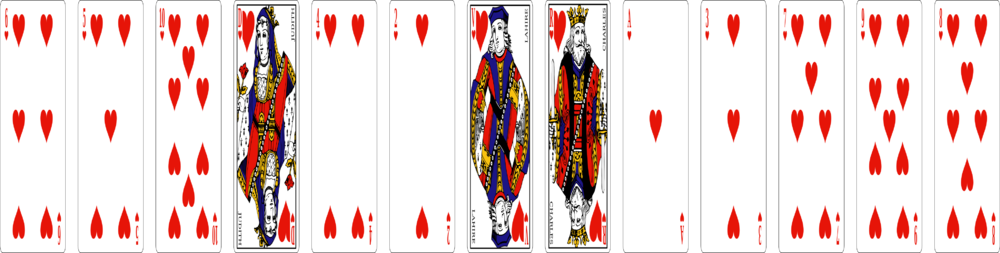
\includegraphics[width=10cm]{ressources/jeu-coeur-melange.png}
    \end{center}
    \begin{center}
        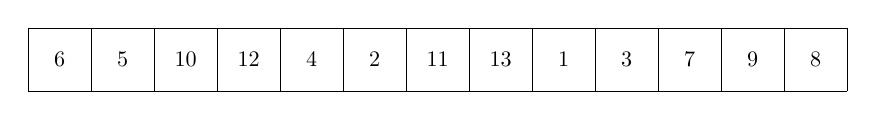
\begin{tikzpicture}[scale=0.8,transform shape]
            \draw (0,0) grid (13,1);
            \foreach \n/\x in {6/0,5/1,10/2,12/3,4/4,2/5,11/6,13/7,1/8,3/9,7/10,9/11,8/12}{
                    \node (\n) at (0.5+\x,0.5) {\n};

                }
        \end{tikzpicture}
        \captionof{figure}{Modélisation}
    \end{center}

\end{frame}
\begin{frame}


    \begin{center}
        \begin{tikzpicture}[scale=0.8,transform shape]
            \draw (0,0) grid (13,1);
            \foreach \n/\x in {6/0,5/1,10/2,12/3,4/4,2/5,11/6,13/7,1/8,3/9,7/10,9/11,8/12}{
                    \node (\n) at (0.5+\x,0.5) {\n};

                }

            \draw[<->,>=latex] (0.5,1) to[bend left=90] (8.5,1);

        \end{tikzpicture}

        \captionof{figure}{Sélection du plus petit élément.}
    \end{center}
    \begin{center}
        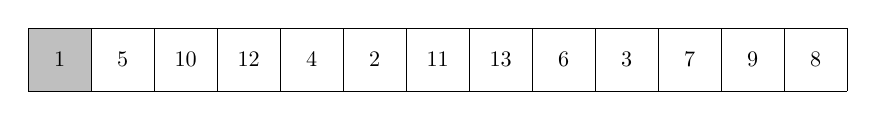
\begin{tikzpicture}[scale=0.8,transform shape]
            \draw (0,0) grid (13,1);
            \draw[fill=gray!50] (0,0)--(1,0)--(1,1)--(0,1)--cycle;
            \foreach \n/\x in {1/0,5/1,10/2,12/3,4/4,2/5,11/6,13/7,6/8,3/9,7/10,9/11,8/12}{
                    \node (\n) at (0.5+\x,0.5) {\n};

                }
        \end{tikzpicture}
        \captionof{figure}{La partie triée est à gauche.}
    \end{center}

\end{frame}
\begin{frame}


    \begin{center}
        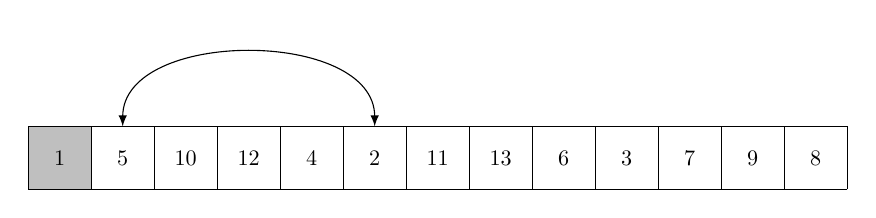
\begin{tikzpicture}[scale=0.8,transform shape]
            \draw (0,0) grid (13,1);
            \draw[fill=gray!50] (0,0)--(1,0)--(1,1)--(0,1)--cycle;
            \foreach \n/\x in {1/0,5/1,10/2,12/3,4/4,2/5,11/6,13/7,6/8,3/9,7/10,9/11,8/12}{
                    \node (\n) at (0.5+\x,0.5) {\n};

                }

            \draw[<->,>=latex] (1.5,1) to[bend left=90] (5.5,1);

        \end{tikzpicture}

        \captionof{figure}{Sélection du plus petit élément.}
    \end{center}
    \begin{center}
        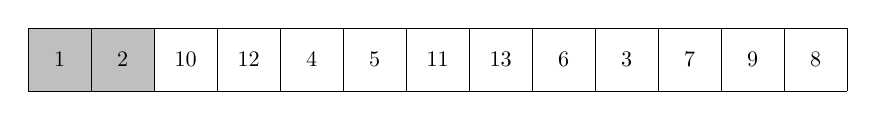
\begin{tikzpicture}[scale=0.8,transform shape]
            \draw[fill=gray!50] (0,0)--(2,0)--(2,1)--(0,1)--cycle;
            \draw (0,0) grid (13,1);
            \foreach \n/\x in {1/0,2/1,10/2,12/3,4/4,5/5,11/6,13/7,6/8,3/9,7/10,9/11,8/12}{
                    \node (\n) at (0.5+\x,0.5) {\n};

                }
        \end{tikzpicture}
        \captionof{figure}{La partie triée est à gauche.}
    \end{center}

\end{frame}
\begin{frame}


    \begin{center}
        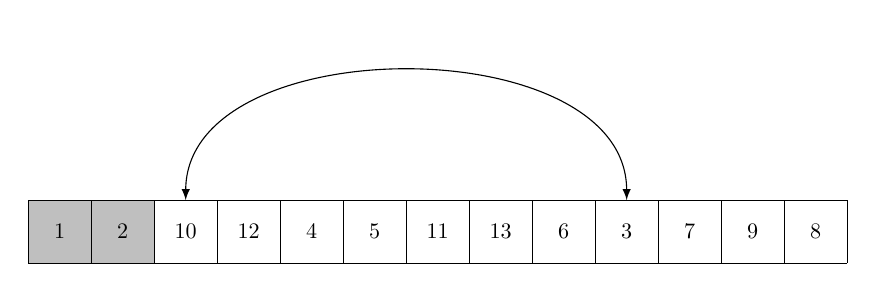
\begin{tikzpicture}[scale=0.8,transform shape]
            \draw[fill=gray!50] (0,0)--(2,0)--(2,1)--(0,1)--cycle;
            \draw (0,0) grid (13,1);

            \foreach \n/\x in {1/0,2/1,10/2,12/3,4/4,5/5,11/6,13/7,6/8,3/9,7/10,9/11,8/12}{
                    \node (\n) at (0.5+\x,0.5) {\n};

                }

            \draw[<->,>=latex] (2.5,1) to[bend left=90] (9.5,1);

        \end{tikzpicture}

        \captionof{figure}{Sélection du plus petit élément.}
    \end{center}
    \begin{center}
        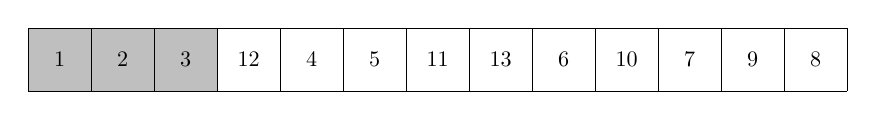
\begin{tikzpicture}[scale=0.8,transform shape]
            \draw[fill=gray!50] (0,0)--(3,0)--(3,1)--(0,1)--cycle;
            \draw (0,0) grid (13,1);
            \foreach \n/\x in {1/0,2/1,3/2,12/3,4/4,5/5,11/6,13/7,6/8,10/9,7/10,9/11,8/12}{
                    \node (\n) at (0.5+\x,0.5) {\n};

                }
        \end{tikzpicture}
        \captionof{figure}{La partie triée est à gauche.}
    \end{center}

\end{frame}
\subsection{Tri par insertion}
\begin{frame}
    \frametitle{Tri par insertion}

    \begin{itemize}
        \item Pour chaque carte du tas:
              \begin{itemize}
                  \item Tant que la carte précédente est plus petite
                  \item Échanger cette carte avec la carte en cours.
              \end{itemize}

    \end{itemize}

\end{frame}
\begin{frame}

    \begin{center}
        \centering
        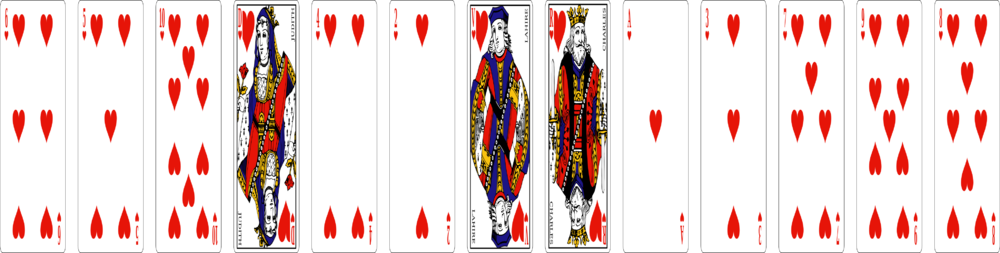
\includegraphics[width=10cm]{ressources/jeu-coeur-melange.png}
    \end{center}
    \begin{center}
        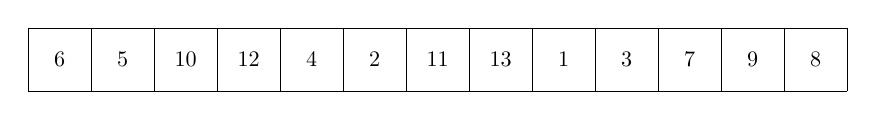
\begin{tikzpicture}[scale=0.8,transform shape]
            \draw (0,0) grid (13,1);
            \foreach \n/\x in {6/0,5/1,10/2,12/3,4/4,2/5,11/6,13/7,1/8,3/9,7/10,9/11,8/12}{
                    \node (\n) at (0.5+\x,0.5) {\n};

                }
        \end{tikzpicture}
        \captionof{figure}{Modélisation}
    \end{center}

\end{frame}
\begin{frame}


    \begin{center}
        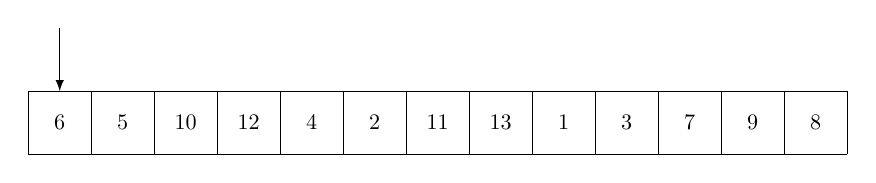
\begin{tikzpicture}[scale=0.8,transform shape]
            \draw (0,0) grid (13,1);
            \foreach \n/\x in {6/0,5/1,10/2,12/3,4/4,2/5,11/6,13/7,1/8,3/9,7/10,9/11,8/12}{
                    \node (\n) at (0.5+\x,0.5) {\n};

                }

            \draw[->,>=latex] (0.5,2) -- (0.5,1);

        \end{tikzpicture}

        \captionof{figure}{Carte en cours}
    \end{center}
    \begin{center}
        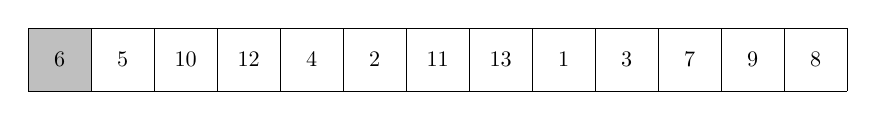
\begin{tikzpicture}[scale=0.8,transform shape]
            \draw[fill=gray!50] (0,0)--(1,0)--(1,1)--(0,1)--cycle;
            \draw (0,0) grid (13,1);

            \foreach \n/\x in {6/0,5/1,10/2,12/3,4/4,2/5,11/6,13/7,1/8,3/9,7/10,9/11,8/12}{
                    \node (\n) at (0.5+\x,0.5) {\n};

                }
        \end{tikzpicture}
        \captionof{figure}{La partie triée est à gauche.}
    \end{center}

\end{frame}
\begin{frame}


    \begin{center}
        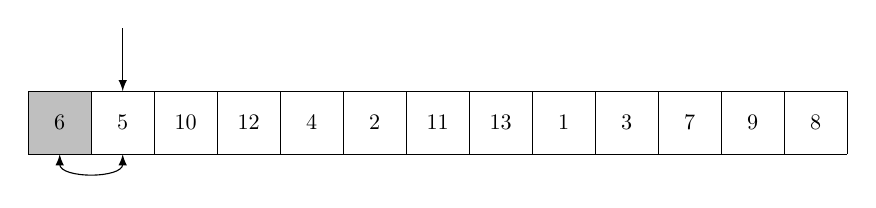
\begin{tikzpicture}[scale=0.8,transform shape]
            \draw[fill=gray!50] (0,0)--(1,0)--(1,1)--(0,1)--cycle;
            \draw (0,0) grid (13,1);
            \foreach \n/\x in {6/0,5/1,10/2,12/3,4/4,2/5,11/6,13/7,1/8,3/9,7/10,9/11,8/12}{
                    \node (\n) at (0.5+\x,0.5) {\n};

                }

            \draw[->,>=latex] (1.5,2) -- (1.5,1);
            \draw[<->,>=latex] (0.5,0) to[bend right=90] (1.5,0);
        \end{tikzpicture}

        \captionof{figure}{Carte en cours}
    \end{center}
    \begin{center}
        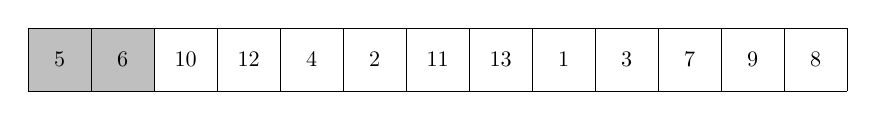
\begin{tikzpicture}[scale=0.8,transform shape]
            \draw[fill=gray!50] (0,0)--(2,0)--(2,1)--(0,1)--cycle;
            \draw (0,0) grid (13,1);

            \foreach \n/\x in {5/0,6/1,10/2,12/3,4/4,2/5,11/6,13/7,1/8,3/9,7/10,9/11,8/12}{
                    \node (\n) at (0.5+\x,0.5) {\n};

                }
        \end{tikzpicture}
        \captionof{figure}{La partie triée est à gauche.}
    \end{center}

\end{frame}
\begin{frame}


    \begin{center}
        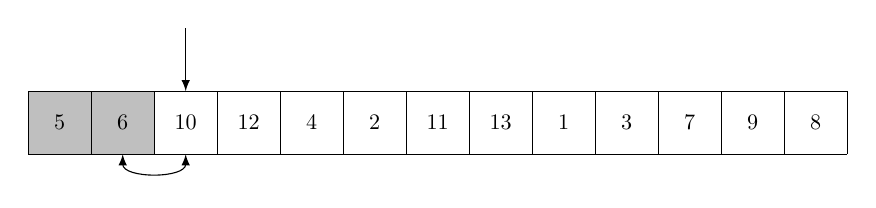
\begin{tikzpicture}[scale=0.8,transform shape]
            \draw[fill=gray!50] (0,0)--(2,0)--(2,1)--(0,1)--cycle;
            \draw (0,0) grid (13,1);
            \foreach \n/\x in {5/0,6/1,10/2,12/3,4/4,2/5,11/6,13/7,1/8,3/9,7/10,9/11,8/12}{
                    \node (\n) at (0.5+\x,0.5) {\n};

                }

            \draw[->,>=latex] (2.5,2) -- (2.5,1);
            \draw[<->,>=latex] (1.5,0) to[bend right=90] (2.5,0);
        \end{tikzpicture}

        \captionof{figure}{Carte en cours}
    \end{center}
    \begin{center}
        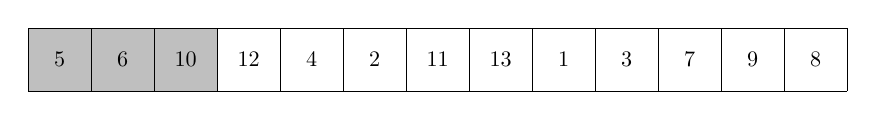
\begin{tikzpicture}[scale=0.8,transform shape]
            \draw[fill=gray!50] (0,0)--(3,0)--(3,1)--(0,1)--cycle;
            \draw (0,0) grid (13,1);

            \foreach \n/\x in {5/0,6/1,10/2,12/3,4/4,2/5,11/6,13/7,1/8,3/9,7/10,9/11,8/12}{
                    \node (\n) at (0.5+\x,0.5) {\n};

                }
        \end{tikzpicture}
        \captionof{figure}{La partie triée est à gauche.}
    \end{center}

\end{frame}
\begin{frame}


    \begin{center}
        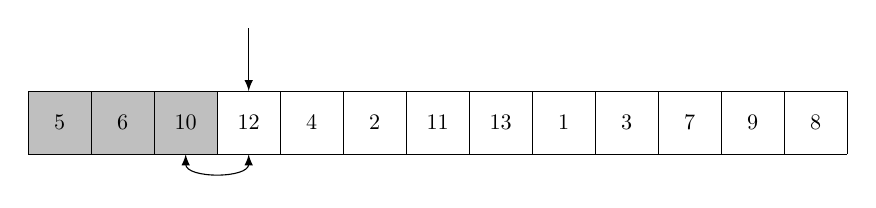
\begin{tikzpicture}[scale=0.8,transform shape]
            \draw[fill=gray!50] (0,0)--(3,0)--(3,1)--(0,1)--cycle;
            \draw (0,0) grid (13,1);
            \foreach \n/\x in {5/0,6/1,10/2,12/3,4/4,2/5,11/6,13/7,1/8,3/9,7/10,9/11,8/12}{
                    \node (\n) at (0.5+\x,0.5) {\n};

                }

            \draw[->,>=latex] (3.5,2) -- (3.5,1);
            \draw[<->,>=latex] (2.5,0) to[bend right=90] (3.5,0);
        \end{tikzpicture}

        \captionof{figure}{Carte en cours}
    \end{center}
    \begin{center}
        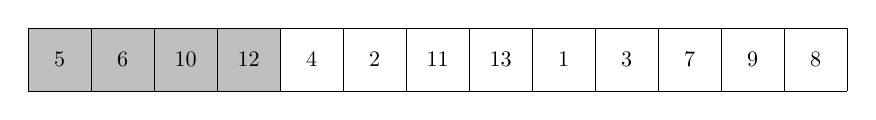
\begin{tikzpicture}[scale=0.8,transform shape]
            \draw[fill=gray!50] (0,0)--(4,0)--(4,1)--(0,1)--cycle;
            \draw (0,0) grid (13,1);

            \foreach \n/\x in {5/0,6/1,10/2,12/3,4/4,2/5,11/6,13/7,1/8,3/9,7/10,9/11,8/12}{
                    \node (\n) at (0.5+\x,0.5) {\n};

                }
        \end{tikzpicture}
        \captionof{figure}{La partie triée est à gauche.}
    \end{center}

\end{frame}
\begin{frame}


    \begin{center}
        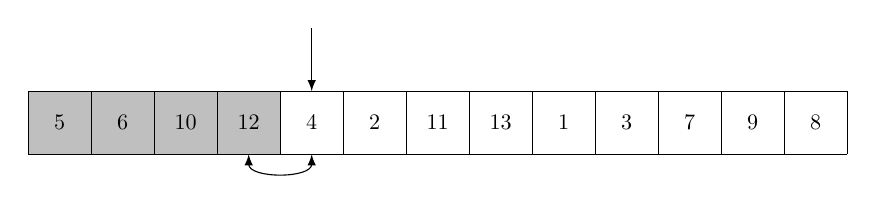
\begin{tikzpicture}[scale=0.8,transform shape]
            \draw[fill=gray!50] (0,0)--(4,0)--(4,1)--(0,1)--cycle;
            \draw (0,0) grid (13,1);
            \foreach \n/\x in {5/0,6/1,10/2,12/3,4/4,2/5,11/6,13/7,1/8,3/9,7/10,9/11,8/12}{
                    \node (\n) at (0.5+\x,0.5) {\n};

                }

            \draw[->,>=latex] (4.5,2) -- (4.5,1);
            \draw[<->,>=latex] (3.5,0) to[bend right=90] (4.5,0);
        \end{tikzpicture}

        \captionof{figure}{Carte en cours}
    \end{center}
    \begin{center}
        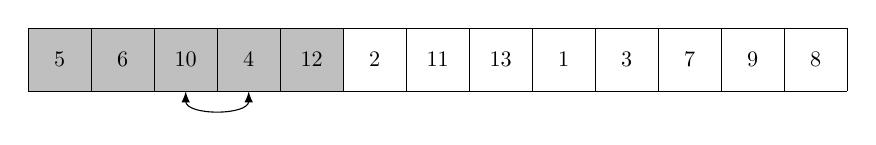
\begin{tikzpicture}[scale=0.8,transform shape]
            \draw[fill=gray!50] (0,0)--(5,0)--(5,1)--(0,1)--cycle;
            \draw (0,0) grid (13,1);

            \foreach \n/\x in {5/0,6/1,10/2,4/3,12/4,2/5,11/6,13/7,1/8,3/9,7/10,9/11,8/12}{
                    \node (\n) at (0.5+\x,0.5) {\n};

                }
            \draw[<->,>=latex] (2.5,0) to[bend right=90] (3.5,0);
        \end{tikzpicture}
        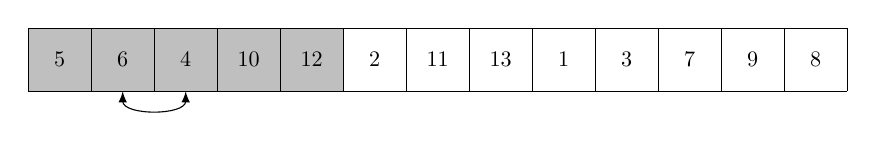
\begin{tikzpicture}[scale=0.8,transform shape]
            \draw[fill=gray!50] (0,0)--(5,0)--(5,1)--(0,1)--cycle;
            \draw (0,0) grid (13,1);

            \foreach \n/\x in {5/0,6/1,4/2,10/3,12/4,2/5,11/6,13/7,1/8,3/9,7/10,9/11,8/12}{
                    \node (\n) at (0.5+\x,0.5) {\n};

                }
            \draw[<->,>=latex] (1.5,0) to[bend right=90] (2.5,0);
        \end{tikzpicture}
        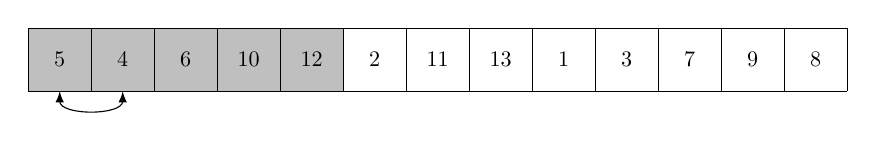
\begin{tikzpicture}[scale=0.8,transform shape]
            \draw[fill=gray!50] (0,0)--(5,0)--(5,1)--(0,1)--cycle;
            \draw (0,0) grid (13,1);

            \foreach \n/\x in {5/0,4/1,6/2,10/3,12/4,2/5,11/6,13/7,1/8,3/9,7/10,9/11,8/12}{
                    \node (\n) at (0.5+\x,0.5) {\n};

                }
            \draw[<->,>=latex] (0.5,0) to[bend right=90] (1.5,0);
        \end{tikzpicture}
        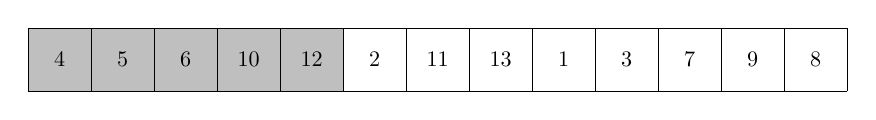
\begin{tikzpicture}[scale=0.8,transform shape]
            \draw[fill=gray!50] (0,0)--(5,0)--(5,1)--(0,1)--cycle;
            \draw (0,0) grid (13,1);

            \foreach \n/\x in {4/0,5/1,6/2,10/3,12/4,2/5,11/6,13/7,1/8,3/9,7/10,9/11,8/12}{
                    \node (\n) at (0.5+\x,0.5) {\n};

                }
        \end{tikzpicture}
        \captionof{figure}{La partie triée est à gauche.}
    \end{center}

\end{frame}
\section{Implémentation}
\subsection{Rappel: Passer un tableau à une fonction}
\begin{frame}[fragile]

    \begin{center}
        \begin{lstlisting}[language=Python]
def ma_fonction(tab: list) -> None:
        tab[2] = 199
        
t = [3, 8, 1, 10, 9]
ma_fonction(t)
\end{lstlisting}
        \captionof{code}{\centering Quand on passe un tableau en argument à une fonction, on passe en réalité \textbf{une référence} au tableau original.}
    \end{center}
    \begin{center}
        \centering
        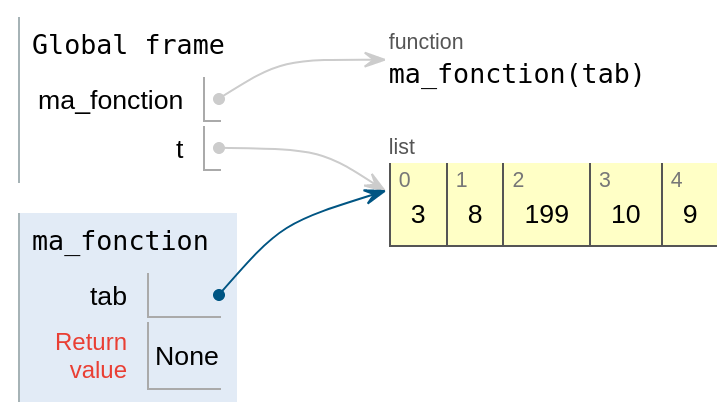
\includegraphics[width=7cm]{ressources/tutor-mutable.png}
        \label{IMG}
    \end{center}
\end{frame}
\subsection{Implémentations des tris}
\begin{frame}
    \frametitle{Implémentation des tris - Tri par sélection}

    \begin{itemize}
        \item Pour chaque carte du tas:
              \begin{itemize}
                  \item \textbf{Trouver la plus petite} carte dans la partie non triée.
                  \item \textbf{Échanger} cette carte avec la première de la partie non triée.
              \end{itemize}

    \end{itemize}

    \begin{activite}
        \begin{enumerate}
            \item Écrire la fonction \textbf{\texttt{indice\_mini(tab: list, dep: int) $\rightarrow$ int}} qui renvoie l'indice de la valeur minimale de \textbf{\texttt{tab}}, entre l'élément d'indice \textbf{\texttt{deb}} et la fin du tableau.
            \item Écrire la fonction \textbf{\texttt{echanger(tab: list, i: int, j: int) $\rightarrow$ None}} qui échange les éléments d'indices \textbf{\texttt{i}} et \textbf{\texttt{j}}.
            \item Écrire alors la fonction \textbf{\texttt{tri\_selection(tab: list) $\rightarrow$ None}}.
        \end{enumerate}
    \end{activite}

\end{frame}
\begin{frame}[fragile]
    \frametitle{Correction}

    \begin{center}
        \begin{lstlisting}[language=Python , basicstyle=\ttfamily\small, xleftmargin=2em, xrightmargin=0em]
def indice_mini(tab: list, dep: int) -> int:
    i_mini = dep
    mini = tab[dep]
    # parcours de la partie du tableau
    for i in range(dep, len(tab)):
        if tab[i] < mini:
            i_mini = i
            mini = tab[i]
    return i_mini
\end{lstlisting}
    \end{center}

\end{frame}
\begin{frame}[fragile]
    \frametitle{Correction}

    \begin{center}
        \begin{lstlisting}[language=Python , basicstyle=\ttfamily\small, xleftmargin=2em, xrightmargin=0em]
def echanger(tab: list, i: int, j: int) -> None:
    temp = tab[i]
    tab[i] = tab[j]
    tab[j] = temp
\end{lstlisting}
    \end{center}

\end{frame}
\begin{frame}[fragile]
    \frametitle{Correction}

    \begin{center}
        \begin{lstlisting}[language=Python , basicstyle=\ttfamily\small, xleftmargin=2em, xrightmargin=0em]
def tri_selection(tab: list) -> None:
    for i in range(len(tab)):
        i_mini = indice_mini(tab, i)
        echanger(tab, i, i_mini)
\end{lstlisting}
    \end{center}

\end{frame}
\begin{frame}
    \frametitle{}

    \begin{activite}
    \begin{enumerate}
        \item Construire par compréhension un tableau de 10 éléments aléatoires compris entre 0 et 100.
        \item Tester alors la fonction de tri.
    \end{enumerate}
    \end{activite}

\end{frame}
\begin{frame}[fragile]
    \frametitle{Correction}

\begin{center}
\begin{lstlisting}[language=Python , basicstyle=\ttfamily\small, xleftmargin=2em, xrightmargin=0em]
t = [randint(0, 100) for _ in range(10)]
print(t)
tri_selection(t)
print(t)
\end{lstlisting}
\end{center}

\end{frame}
\begin{frame}
    \frametitle{Tri par insertion}
    \begin{itemize}
        \item Pour chaque carte du tas:
              \begin{itemize}
                  \item Tant que la carte précédente est plus petite
                  \item \textbf{Échanger} cette carte avec la carte en cours.
              \end{itemize}

    \end{itemize}
    \begin{activite}
        \begin{enumerate}
            \item Écrire la fonction \textbf{\texttt{inserer(tab: list, j: int) $\rightarrow$ None}} qui insère l'élément de rang \textbf{\texttt{j}} dans la partie déjà triée.
            \item Écrire alors la fonction \textbf{\texttt{tri\_insertion(tab: list) $\rightarrow$ None}}.
        \end{enumerate}
    \end{activite}

\end{frame}
\begin{frame}[fragile]
    \frametitle{Correction}

\begin{center}
\begin{lstlisting}[language=Python , basicstyle=\ttfamily\small, xleftmargin=2em, xrightmargin=0em]
def inserer(tab: list, j: int) -> None:
    while j-1 >= 0 and tab[j-1] > tab[j]:
        echanger(tab, j-1, j)
        j = j-1
\end{lstlisting}
\end{center}
\begin{aretenir}[Remarque]
La condition \textbf{\texttt{j-1 >= 0}} évite de \emph{sortir} du tableau.
\end{aretenir}
\end{frame}
\begin{frame}[fragile]
    \frametitle{}

\begin{center}
\begin{lstlisting}[language=Python , basicstyle=\ttfamily\small, xleftmargin=2em, xrightmargin=0em]
def tri_insertion(tab: list) -> None:
    for i in range(len(tab)):
        inserer(tab, i)
\end{lstlisting}
\end{center}

\end{frame}
\section{Études des implémentations}
\subsection{Terminaison}
\begin{frame}
    \frametitle{Études: Terminaison}

\begin{aretenir}[]
Pour montrer que l'algorithme termine (ne part pas dans une boucle sans fin), on utilise \textbf{un variant de boucle}.
\end{aretenir}

\end{frame}
\begin{frame}
    \frametitle{Tri par sélection}

    Pour le tri par sélection, on utilise deux boucles \textbf{bornées}. La terminaison est dans ce cas évidente: les deux boucles s'arrêteront obligatoirement.

\end{frame}
\begin{frame}[fragile]
    \frametitle{Tri par insertion}
Pour le tri par insertion:
\begin{center}
\begin{lstlisting}[language=Python , basicstyle=\ttfamily\small, xleftmargin=2em, xrightmargin=0em]
def inserer(tab: list, j: int) -> None:
    while j-1 >= 0 and tab[j-1] > tab[j]:
        echanger(tab, j-1, j)
        j = j-1
\end{lstlisting}
\captionof{code}{La fonction \textbf{\texttt{inserer}} contient une boucle non bornée.}
\label{CODE}
\end{center}
    \begin{itemize}
        \item La variable \textbf{\texttt{j}} est un variant de boucle. 
        \item ligne 4: À chaque tour, \textbf{\texttt{j}} est diminué de 1.
        \item ligne 1: L'instruction \textbf{\texttt{j-1 >= 0}} assure que la boucle se termine.
    \end{itemize}

\end{frame}
\subsection{Correction}
\begin{frame}
    \frametitle{Correction}

    \begin{aretenir}[]
    Pour montrer que l'algorithme est correct, on utilise \textbf{un invariant de boucle}. Un invariant est une expression qui reste vraie à chaque itération de boucle.
    \end{aretenir}

\end{frame}
\begin{frame}
    \frametitle{Tri par sélection}

    Pour le tri par sélection, l'invariant de boucle est:
    \begin{framed}\centering
        Avant chaque itération de la boucle externe, la partie gauche du tableau est triée.
    \end{framed}
    \begin{center}
        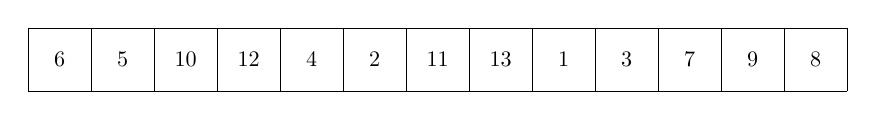
\begin{tikzpicture}[scale=0.8,transform shape]
            \draw (0,0) grid (13,1);
            \foreach \n/\x in {6/0,5/1,10/2,12/3,4/4,2/5,11/6,13/7,1/8,3/9,7/10,9/11,8/12}{
                    \node (\n) at (0.5+\x,0.5) {\n};

                }
        \end{tikzpicture}
        \captionof{figure}{Vraie avant la première itération.}
    \end{center}
\end{frame}
\begin{frame}
    \frametitle{}

    \begin{center}
        \begin{tikzpicture}[scale=0.8,transform shape]
            \draw (0,0) grid (13,1);
            \foreach \n/\x in {6/0,5/1,10/2,12/3,4/4,2/5,11/6,13/7,1/8,3/9,7/10,9/11,8/12}{
                    \node (\n) at (0.5+\x,0.5) {\n};

                }

            \draw[<->,>=latex] (0.5,1) to[bend left=90] (8.5,1);

        \end{tikzpicture}
    \end{center}
    \begin{center}
        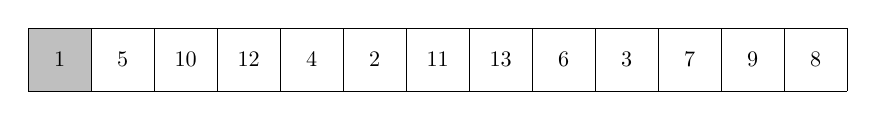
\begin{tikzpicture}[scale=0.8,transform shape]
            \draw (0,0) grid (13,1);
            \draw[fill=gray!50] (0,0)--(1,0)--(1,1)--(0,1)--cycle;
            \foreach \n/\x in {1/0,5/1,10/2,12/3,4/4,2/5,11/6,13/7,6/8,3/9,7/10,9/11,8/12}{
                    \node (\n) at (0.5+\x,0.5) {\n};

                }
        \end{tikzpicture}
        \captionof{figure}{Vraie avant la deuxième itération.}
    \end{center}

\end{frame}
\begin{frame}


    \begin{center}
        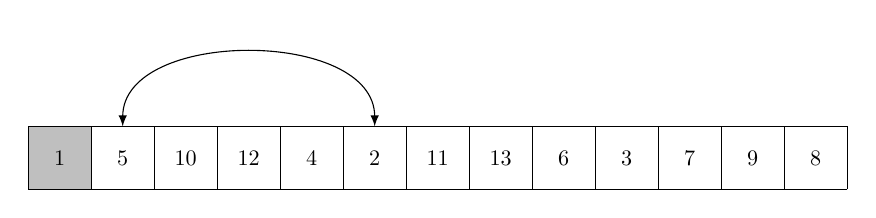
\begin{tikzpicture}[scale=0.8,transform shape]
            \draw (0,0) grid (13,1);
            \draw[fill=gray!50] (0,0)--(1,0)--(1,1)--(0,1)--cycle;
            \foreach \n/\x in {1/0,5/1,10/2,12/3,4/4,2/5,11/6,13/7,6/8,3/9,7/10,9/11,8/12}{
                    \node (\n) at (0.5+\x,0.5) {\n};

                }

            \draw[<->,>=latex] (1.5,1) to[bend left=90] (5.5,1);

        \end{tikzpicture}
    \end{center}
    \begin{center}
        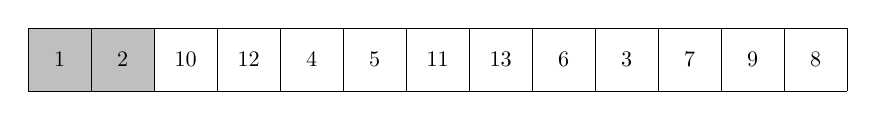
\begin{tikzpicture}[scale=0.8,transform shape]
            \draw[fill=gray!50] (0,0)--(2,0)--(2,1)--(0,1)--cycle;
            \draw (0,0) grid (13,1);
            \foreach \n/\x in {1/0,2/1,10/2,12/3,4/4,5/5,11/6,13/7,6/8,3/9,7/10,9/11,8/12}{
                    \node (\n) at (0.5+\x,0.5) {\n};

                }
        \end{tikzpicture}
        \captionof{figure}{Vraie avant la troisième itération.}
    \end{center}
\begin{aretenir}[]
On peut démontrer que la relation est vraie pour n'importe quelle itération.
\end{aretenir}
\end{frame}
\begin{frame}
    \frametitle{Tri par insertion}

    Pour le tri par insertion, l'invariant de boucle est le même:
    \begin{framed}\centering
        Avant chaque itération de la boucle externe, la partie gauche du tableau est triée.
    \end{framed}
    \begin{center}
        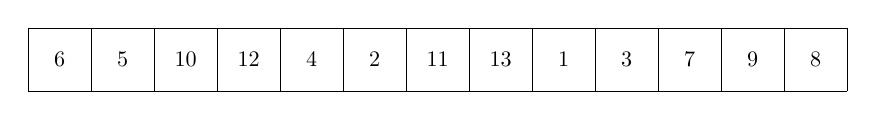
\begin{tikzpicture}[scale=0.8,transform shape]
            \draw (0,0) grid (13,1);
            \foreach \n/\x in {6/0,5/1,10/2,12/3,4/4,2/5,11/6,13/7,1/8,3/9,7/10,9/11,8/12}{
                    \node (\n) at (0.5+\x,0.5) {\n};

                }
        \end{tikzpicture}
        \captionof{figure}{Vraie avant la première itération.}
    \end{center}
\end{frame}
\begin{frame}


    \begin{center}
        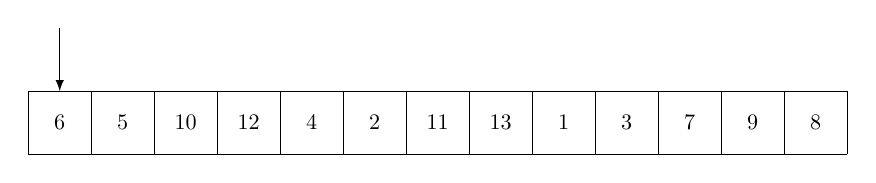
\begin{tikzpicture}[scale=0.8,transform shape]
            \draw (0,0) grid (13,1);
            \foreach \n/\x in {6/0,5/1,10/2,12/3,4/4,2/5,11/6,13/7,1/8,3/9,7/10,9/11,8/12}{
                    \node (\n) at (0.5+\x,0.5) {\n};

                }

            \draw[->,>=latex] (0.5,2) -- (0.5,1);

        \end{tikzpicture}
    \end{center}
    \begin{center}
        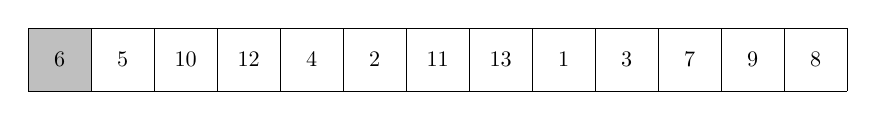
\begin{tikzpicture}[scale=0.8,transform shape]
            \draw[fill=gray!50] (0,0)--(1,0)--(1,1)--(0,1)--cycle;
            \draw (0,0) grid (13,1);

            \foreach \n/\x in {6/0,5/1,10/2,12/3,4/4,2/5,11/6,13/7,1/8,3/9,7/10,9/11,8/12}{
                    \node (\n) at (0.5+\x,0.5) {\n};

                }
        \end{tikzpicture}
        \captionof{figure}{Vraie avant la deuxième itération.}
    \end{center}

\end{frame}
\begin{frame}


    \begin{center}
        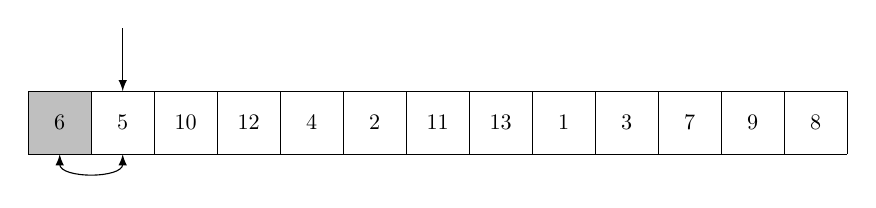
\begin{tikzpicture}[scale=0.8,transform shape]
            \draw[fill=gray!50] (0,0)--(1,0)--(1,1)--(0,1)--cycle;
            \draw (0,0) grid (13,1);
            \foreach \n/\x in {6/0,5/1,10/2,12/3,4/4,2/5,11/6,13/7,1/8,3/9,7/10,9/11,8/12}{
                    \node (\n) at (0.5+\x,0.5) {\n};

                }

            \draw[->,>=latex] (1.5,2) -- (1.5,1);
            \draw[<->,>=latex] (0.5,0) to[bend right=90] (1.5,0);
        \end{tikzpicture}
    \end{center}
    \begin{center}
        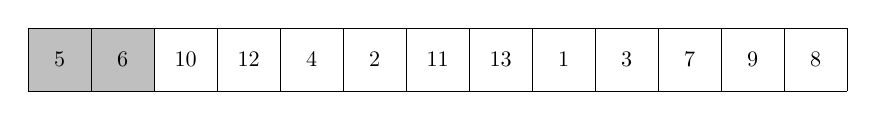
\begin{tikzpicture}[scale=0.8,transform shape]
            \draw[fill=gray!50] (0,0)--(2,0)--(2,1)--(0,1)--cycle;
            \draw (0,0) grid (13,1);

            \foreach \n/\x in {5/0,6/1,10/2,12/3,4/4,2/5,11/6,13/7,1/8,3/9,7/10,9/11,8/12}{
                    \node (\n) at (0.5+\x,0.5) {\n};

                }
        \end{tikzpicture}
        \captionof{figure}{Vraie avant la troisième itération.}
    \end{center}
    \begin{aretenir}[]
        On peut démontrer que la relation est vraie pour n'importe quelle itération.
        \end{aretenir}
\end{frame}
\subsection{Complexité}
\begin{frame}
    \frametitle{Complexité}

    \begin{aretenir}[]
    \begin{itemize}
        \item La complexité étudie les performances d'un algorithme. 
        \item Elles sont indépendantes de la puissance de la machine. 
        \item On étudie le nombre d'opérations que doit effectuer l'algorithme.
    \end{itemize}
    \end{aretenir}

\end{frame}
\begin{frame}[fragile]
    \frametitle{Tri par sélection}

\begin{center}
\begin{lstlisting}[language=Python , basicstyle=\ttfamily\small, xleftmargin=2em, xrightmargin=0em]
def tri_selection(tab: list) -> None:
    for i in range(len(tab)):
        i_mini = indice_mini(tab, i)
        echanger(tab, i, i_mini)
\end{lstlisting}
\end{center}

\begin{aretenir}[Observation]
On note \textbf{\texttt{n}} la taille du tableau.\\La boucle (ligne 2) effectue \textbf{\texttt{n}} itérations.
\end{aretenir}
\end{frame}
\begin{frame}[fragile]
    \frametitle{}

\begin{center}
\begin{lstlisting}[language=Python , basicstyle=\ttfamily\small, xleftmargin=2em, xrightmargin=0em]
def tri_selection(tab: list) -> None:
    for i in range(len(tab)):
        i_mini = indice_mini(tab, i)
        echanger(tab, i, i_mini)
\end{lstlisting}
\begin{lstlisting}[language=Python , basicstyle=\ttfamily\small, xleftmargin=2em, xrightmargin=0em]
def indice_mini(tab: list, dep: int) -> int:
    i_mini = dep
    mini = tab[dep]
    for i in range(dep, len(tab)):
        if tab[i] < mini:
            i_mini = i
            mini = tab[i]
    return i_mini
\end{lstlisting}
\end{center}
\begin{aretenir}[Observation]
À chaque itération, la fonction de tri appelle la fonction \textbf{\texttt{indice\_mini}}. Cette dernière effectue \textbf{\texttt{n-dep}} itérations.
\end{aretenir}
\end{frame}
\begin{frame}[fragile]
    \begin{itemize}
        \item à la première itération de \textbf{\texttt{i}}, la boucle de \textbf{\texttt{indice\_mini}} effectue \textbf{\texttt{n-1}} itérations.
        \begin{center}
            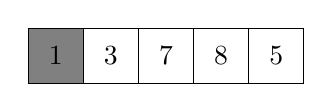
\begin{tikzpicture}[scale=0.7]        
                \fill[gray] (0,0) -- (1,0) -- (1,1) -- (0,1)-- cycle;
                \draw (0,0) grid (5,1);
                \node at(0.5,0.5) {1};
                \node at(1.5,0.5) {3};
                \node at(2.5,0.5) {7};
                \node at(3.5,0.5) {8};
                \node at(4.5,0.5) {5};
        
            \end{tikzpicture}
            \end{center}
        \item à la deuxième itération de \textbf{\texttt{i}}, la boucle de \textbf{\texttt{indice\_mini}} effectue \textbf{\texttt{n-2}} itérations.
        \begin{center}
            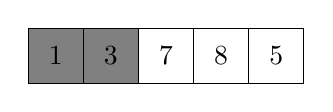
\begin{tikzpicture}[scale=0.7]        
                \fill[gray] (0,0) -- (2,0) -- (2,1) -- (0,1)-- cycle;
                \draw (0,0) grid (5,1);
                \node at(0.5,0.5) {1};
                \node at(1.5,0.5) {3};
                \node at(2.5,0.5) {7};
                \node at(3.5,0.5) {8};
                \node at(4.5,0.5) {5};
        
            \end{tikzpicture}
            \end{center}
        \item \dots
    \end{itemize}
    
\end{frame}
\begin{frame}
    \frametitle{}
    $$\sum_{k=1}^{n-1}{k}=(n-1)+(n-2)+\dots+2+1=\dfrac{n.(n-1)}{2}$$
    \note{démo 2 colonnes inversées de 1+2+...+n-1}
    \begin{aretenir}[]
        Le tri par sélection effectue $\dfrac{n.(n-1)}{2}$ opérations pour ordonner le tableau. 
        
        \centering Le nombre d'opérations dépend de $n^2$. On dit que la complexité est \textbf{quadratique}.
    \end{aretenir}

\end{frame}
\begin{frame}
    \frametitle{Évolution du nombre d'itérations}

    \begin{center}
    \centering
    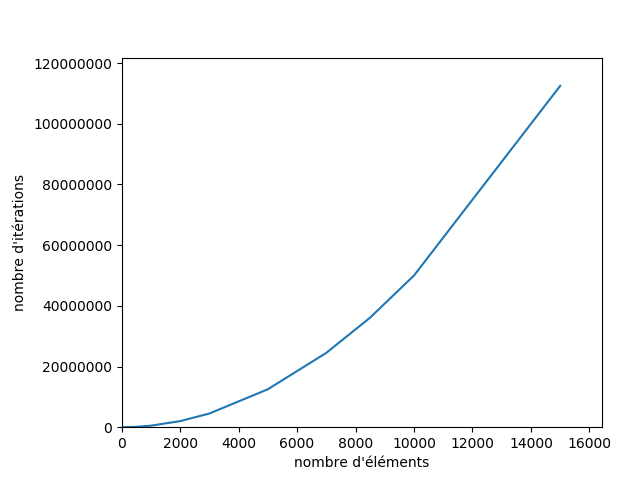
\includegraphics[width=10cm]{ressources/complexite-selection.png}
    \end{center}
\note{15000 éléments $\rightarrow$ 100 millions d'itérations}
\end{frame}
\begin{frame}[fragile]
    \frametitle{Tri par insertion}

\begin{center}
\begin{lstlisting}[language=Python , basicstyle=\ttfamily\small, xleftmargin=2em, xrightmargin=0em]
def tri_insertion(tab: list) -> None:
    for i in range(len(tab)):
        inserer(tab, i)
\end{lstlisting}
\end{center}   
\begin{aretenir}[Observation]
On note \textbf{\texttt{n}} la taille du tableau.\\La boucle (ligne 2) effectue \textbf{\texttt{n}} itérations.
\end{aretenir}  
\end{frame}
\begin{frame}[fragile]
    \frametitle{}

\begin{center}
\begin{lstlisting}[language=Python , basicstyle=\ttfamily\small, xleftmargin=2em, xrightmargin=0em]
def tri_insertion(tab: list) -> None:
    for i in range(len(tab)):
        inserer(tab, i)
\end{lstlisting}
\begin{lstlisting}[language=Python , basicstyle=\ttfamily\small, xleftmargin=2em, xrightmargin=0em]
def inserer(tab: list, j: int) -> None:
    while j-1 >= 0 and tab[j-1] > tab[j]:
        echanger(tab, j-1, j)
        j = j-1
\end{lstlisting}
\end{center}   
\begin{aretenir}[Observation]
À chaque itération, la fonction de tri appelle la fonction \textbf{\texttt{inserer}}. Le nombre d'itérations de la boucle \textbf{\texttt{while}} peut varier.
\end{aretenir}
\end{frame}
\begin{frame}[fragile]
    \frametitle{}
\begin{center}
\begin{lstlisting}[language=Python , basicstyle=\ttfamily\small, xleftmargin=2em, xrightmargin=0em]
def inserer(tab: list, j: int) -> None:
    while j-1 >= 0 and tab[j-1] > tab[j]:
        echanger(tab, j-1, j)
        j = j-1
\end{lstlisting}
\end{center} 
    \begin{center}
        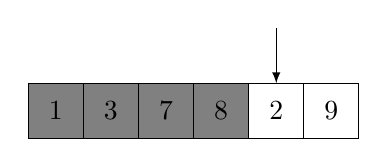
\begin{tikzpicture}[scale=0.7]        
            \fill[gray] (0,0) -- (4,0) -- (4,1) -- (0,1)-- cycle;
            \draw (0,0) grid (6,1);
            \node at(0.5,0.5) {1};
            \node at(1.5,0.5) {3};
            \node at(2.5,0.5) {7};
            \node at(3.5,0.5) {8};
            \node at(4.5,0.5) {2};
            \node at(5.5,0.5) {9};    
            \draw[->,>=latex] (4.5,2) -- (4.5,1);

        \end{tikzpicture}
        \captionof{figure}{3 itérations pour placer \textbf{\texttt{2}}}
        \end{center} 
        \begin{center}
            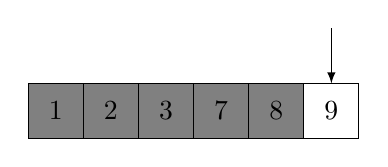
\begin{tikzpicture}[scale=0.7]        
                \fill[gray] (0,0) -- (5,0) -- (5,1) -- (0,1)-- cycle;
                \draw (0,0) grid (6,1);
            \node at(0.5,0.5) {1};
            \node at(1.5,0.5) {2};
            \node at(2.5,0.5) {3};
            \node at(3.5,0.5) {7};
            \node at(4.5,0.5) {8};
            \node at(5.5,0.5) {9};     
                \draw[->,>=latex] (5.5,2) -- (5.5,1);
    
            \end{tikzpicture}
            \captionof{figure}{0 itération pour placer \textbf{\texttt{9}}}
            \end{center} 
\end{frame}
\begin{frame}
    \frametitle{}

    \begin{activite}
        \begin{enumerate}
            \item Compter le nombre d'itérations de la boucle \textbf{\texttt{while}} si le tableau est déjà trié.
            \item Compter le nombre d'itérations de la boucle \textbf{\texttt{while}} si le tableau est trié dans l'ordre décroissant.
        \end{enumerate}
    \end{activite}

\end{frame}
\begin{frame}[fragile]
    \frametitle{Correction}

    \begin{center}
\begin{lstlisting}[language=Python , basicstyle=\ttfamily\small, xleftmargin=2em, xrightmargin=0em]
def inserer(tab: list, j: int) -> None:
    while j-1 >= 0 and tab[j-1] > tab[j]:
        echanger(tab, j-1, j)
        j = j-1
\end{lstlisting}
        \end{center}
    \begin{center}
        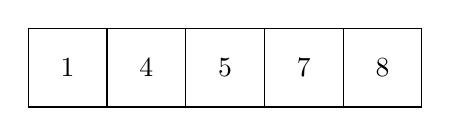
\begin{tikzpicture}  
            \draw (0,-2) grid (5,-1);
            \node at(0.5,-1.5) {1};
            \node at(1.5,-1.5) {4};
            \node at(2.5,-1.5) {5};
            \node at(3.5,-1.5) {7};
            \node at(4.5,-1.5) {8};
        \end{tikzpicture}
        \captionof{code}{Le tableau est déjà trié. La boucle \textbf{\texttt{while}} n'effectue aucune itération.}
        \label{CODE}
        \end{center}

\end{frame}

\begin{frame}[fragile]
    \frametitle{Correction}

\begin{center}
\begin{lstlisting}[language=Python , basicstyle=\ttfamily\small, xleftmargin=2em, xrightmargin=0em]
def inserer(tab: list, j: int) -> None:
    while j-1 >= 0 and tab[j-1] > tab[j]:
        echanger(tab, j-1, j)
        j = j-1
\end{lstlisting}
\end{center}
    \begin{center}
        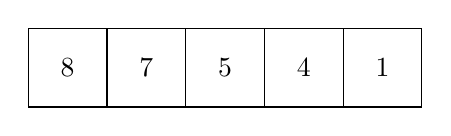
\begin{tikzpicture} 
            \draw (0,-2) grid (5,-1);
            \node at(0.5,-1.5) {8};
            \node at(1.5,-1.5) {7};
            \node at(2.5,-1.5) {5};
            \node at(3.5,-1.5) {4};
            \node at(4.5,-1.5) {1};
        \end{tikzpicture}
        \captionof{code}{Le tableau est inversé. La boucle \textbf{\texttt{wile}} effectue \textbf{\texttt{i}} itérations.}
        \label{CODE}
        \end{center}

\end{frame}
\begin{frame}
    \frametitle{}

    \begin{aretenir}[]
    \begin{itemize}
        \item<1-> Dans le meilleur des cas (tableau déjà trié), la boucle imbriquée \textbf{\texttt{while}} effectue \textbf{\texttt{0}} itération. Dans ce cas particulier, le tri par insertion est en temps \textbf{linéaire}.
        \item<2-> Dans le pire des cas (tableau inversé), la boucle imbriquée \textbf{\texttt{while}} effectue \textbf{\texttt{n}} itérations. Le tri par insertion est en temps \textbf{quadratique} ($n^2$).
        \item<3-> En moyenne (tableau quelconque), la boucle imbriquée effectue \textbf{\texttt{n}} itérations. Le tri par insertion est en temps \textbf{quadratique} ($n^2$).
    \end{itemize}
    \end{aretenir}

\end{frame}
\end{document}